\documentclass[12pt]{article}
\usepackage[a4paper, margin=1in]{geometry} 
\usepackage{graphicx} 
\usepackage{hyperref}
\usepackage{float}
\usepackage{multicol}
\usepackage{multirow}
\usepackage{amsmath}
\usepackage[ruled]{algorithm2e}
\usepackage{amssymb}
\usepackage[font=small, labelfont=bf]{caption}

\title{Lecture Notes for \\ INF281 Basics of Bioinformatics Sequence Analysis}
\author{Takaya Saito}
\date{}

\begin{document}

\pagenumbering{arabic}
\setcounter{page}{36}

\makeatletter 
\renewcommand{\thefigure}{\arabic{section}.\arabic{figure}}
\renewcommand{\thetable}{\arabic{section}.\arabic{table}}
\makeatother

%
% Database search
%
\setcounter{section}{5}
\setcounter{figure}{0}
\setcounter{table}{0}
\section{Database search}
%\documentclass[12pt]{article}
%\usepackage[a4paper, margin=1in]{geometry} 
%\usepackage{graphicx} 
%\usepackage{hyperref}
%\usepackage{float}
%\usepackage{multicol}
%\usepackage{multirow}
%\usepackage[font=small, labelfont=bf]{caption}
%
%\begin{document}

%
% Biological databases
%
 \subsection{Biological databases}
Biological databases contain biological information, mainly collected from molecular biology experiments, life science literature, and bioinformatics analyses.

%
% Categories of databases
%
\subsubsection*{Categories of databases} 
Annual \href{http://nar.oxfordjournals.org}{Nucleic Acids Research} database issue includes the following database categories.

\begin{itemize}
\item Nucleotide Sequence Databases
\item RNA sequence databases
\item Protein sequence databases
\item Structure Databases
\item Proteomics Resources
\item Human and other Vertebrate Genomes
\item Genomics Databases (non-vertebrate)
\item Plant databases
\item Human Genes and Diseases
\item Metabolic and Signaling Pathways
\item Immunological databases
\item ...
\end{itemize}

%
% GenBank
%
\subsubsection*{GenBank} 
\begin{itemize}
\item A comprehensive database of publicly available nucleotide sequences
\item Produced and maintained by NCBI (National Center for Biotechnology Information, URL: \href{http://www.ncbi.nlm.nih.gov}{http://www.ncbi.nlm.nih.gov})
\end{itemize}

\begin{figure}[H]
  \centering
      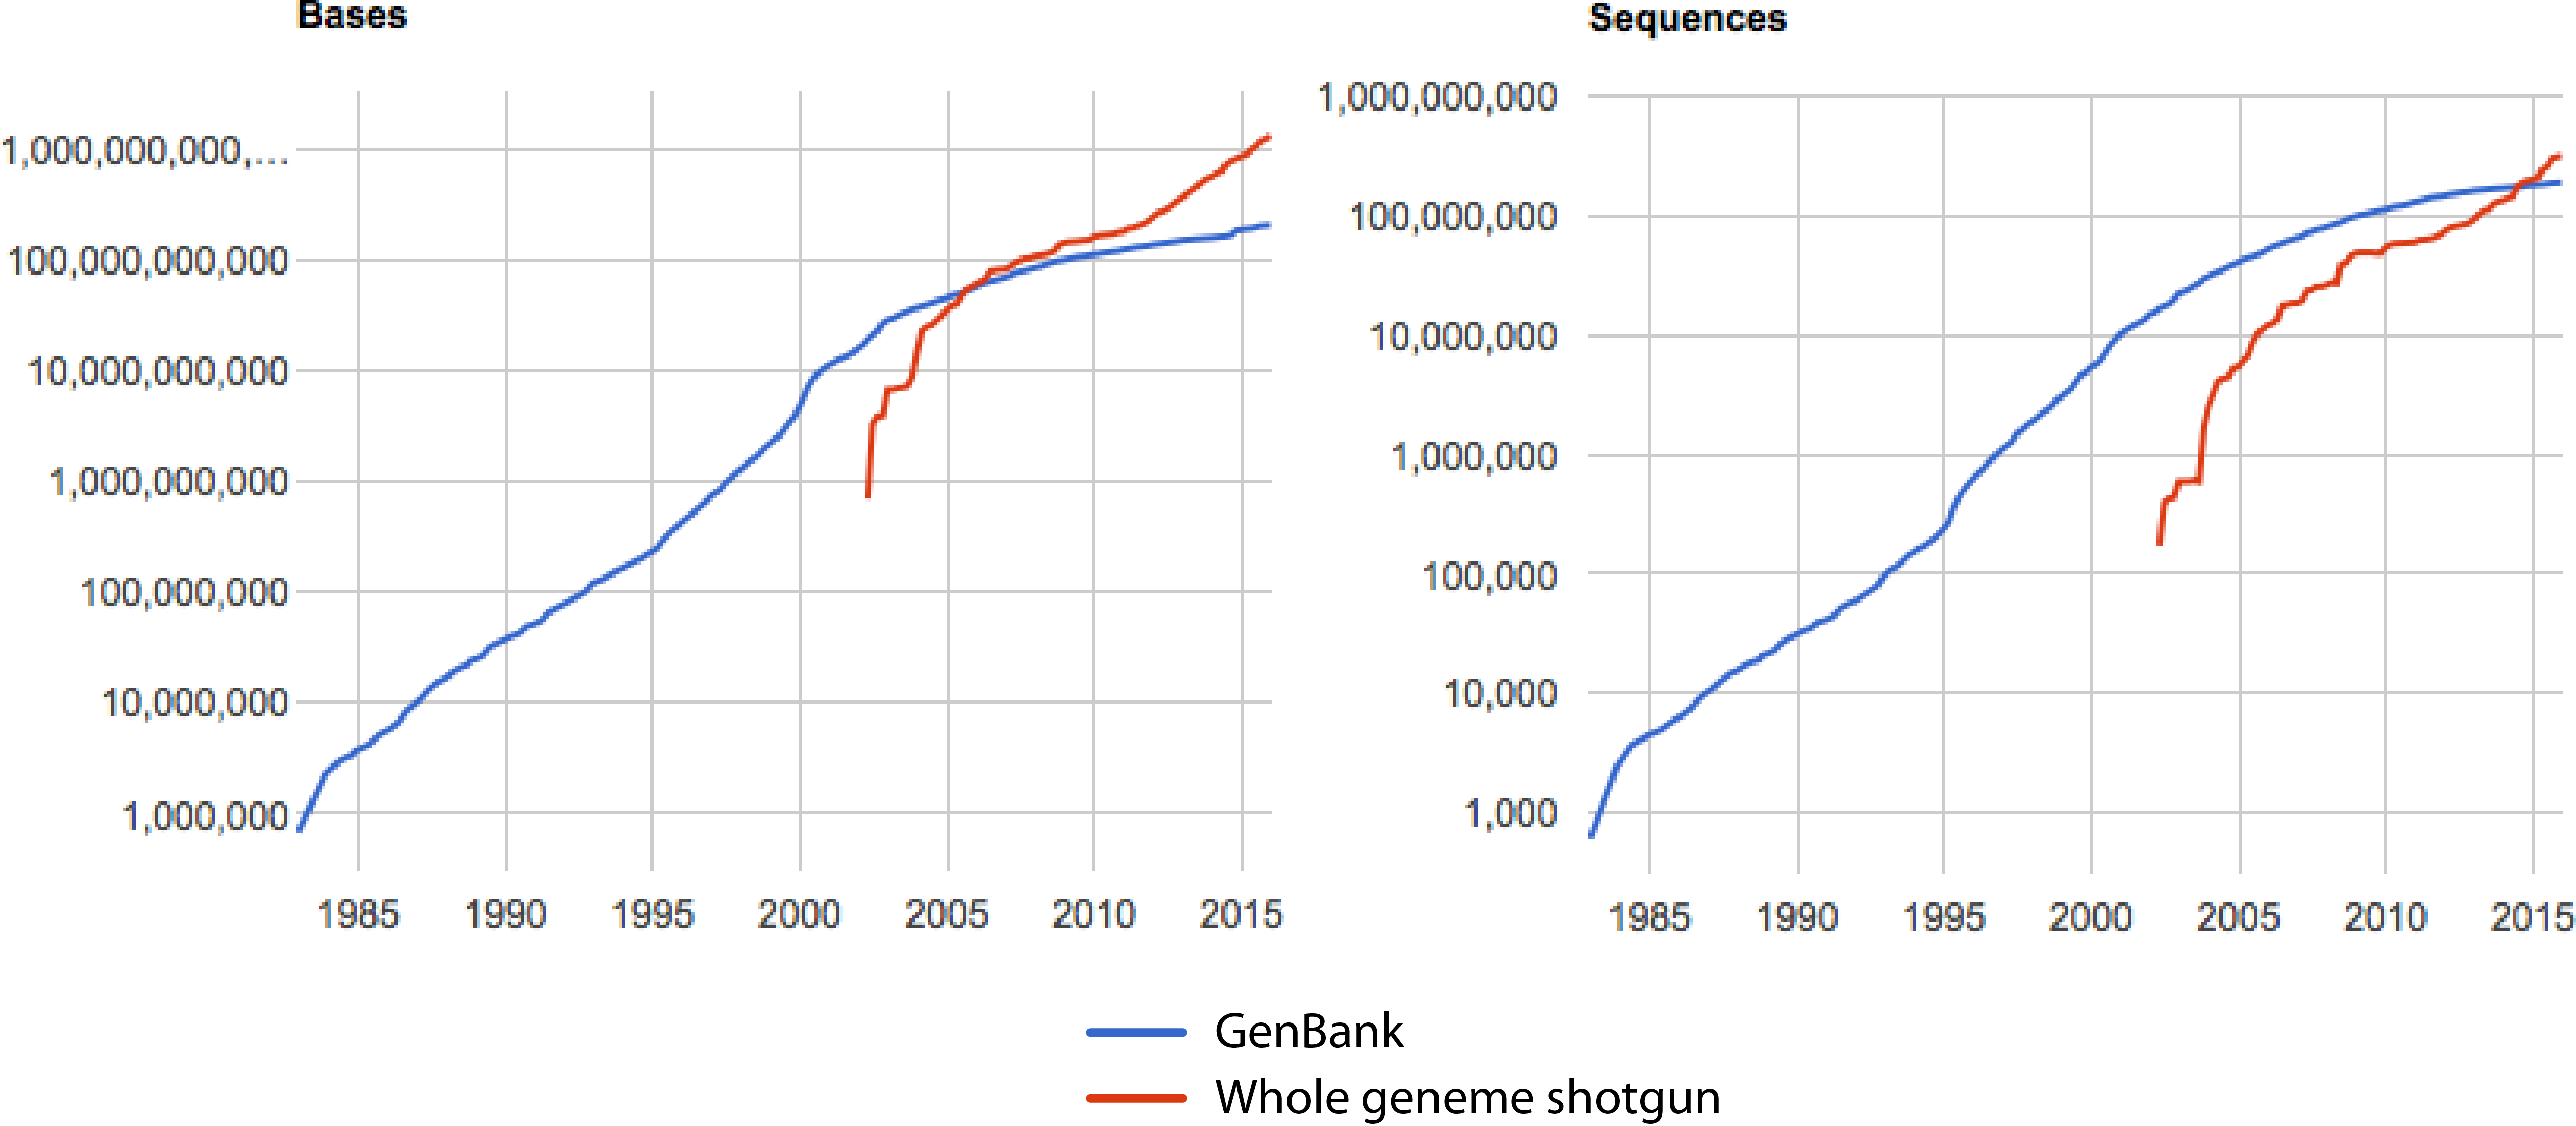
\includegraphics[width=0.6 \textwidth]{fig05/genebank_stat.png}
  \caption{Growth of GenBank and WGS (source: \href{http://www.ncbi.nlm.nih.gov/genbank/statistics}{NCBI})}
\end{figure}

%
% UniProt
%
\subsubsection*{UniProt} 
\begin{itemize}
\item A central repository of protein data from Swiss-Prot, TrEMBL, and PIR-PSD databases
\item Maintained by the UniProt consortium
\end{itemize}

%
% Sequence data 
%
\subsubsection*{Sequence data} 
\begin{itemize}
\item Identifier
\item Sequence
\end{itemize}

\noindent
\textbf{Data format of sequence data} \\
FASTA is the most popular format for sequence data.
\begin{figure}[H]
  \centering
      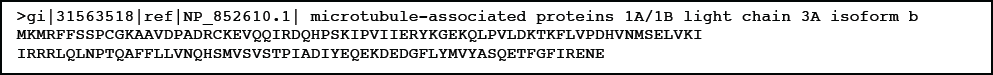
\includegraphics[width=\textwidth]{fig05/fasta.png}
\end{figure}

%
% Annotation data
%
\subsubsection*{Annotation data} 
Sequences databases usually contain annotations in addition to sequences. 

\begin{itemize}
\item Notes and descriptions of important regions and components
\item Meta data
\end{itemize}

\noindent
\textbf{Data format of annotation data} \\
Annotation data can be downloaded in many different formats. GFF is one of the popular file formats for storing genomic features.
\begin{figure}[H]
  \centering
      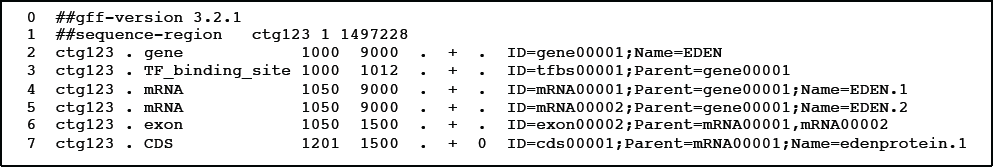
\includegraphics[width=\textwidth]{fig05/gff3.png}
\end{figure}

%
% Tools
%
\subsubsection*{Tools}
Many database tools are available for various purposes.
 
\noindent
\textbf{Search tools for sequence databases}
\begin{itemize}
\item BLAST at NCBI (\href{http://blast.ncbi.nlm.nih.gov/Blast.cgi}{http://blast.ncbi.nlm.nih.gov/Blast.cgi})
\item BLAT/BLAST at Ensembl (\href{http://www.ensembl.org/Multi/Tools/Blast}{http://www.ensembl.org/Multi/Tools/Blast})
\end{itemize}

\noindent
\textbf{Data browsing tools of annotation and sequence data}
\begin{itemize}
\item UCSC Genome Browser (\href{https://genome.ucsc.edu}{https://genome.ucsc.edu})
\item Ensemble Genome Browser (\href{http://www.ensembl.org}{http://www.ensembl.org})
\end{itemize}

\noindent
\textbf{Data download tools for annotation and sequence data}
\begin{itemize}
\item UCSC Table Browser (\href{http://genome.ucsc.edu/cgi-bin/hgTables}{http://genome.ucsc.edu/cgi-bin/hgTables})
\item Ensemble BioMart (\href{http://www.ensembl.org/biomart}{http://www.ensembl.org/biomart})
\end{itemize}

\noindent
\textbf{Tools for protein data}
\begin{itemize}
\item UniProt (\href{https://www.uniprot.org}{https://www.uniprot.org})
\end{itemize}

\bigskip 

%\end{document}

%\documentclass[12pt]{article}
%\usepackage[a4paper, margin=1in]{geometry} 
%\usepackage{graphicx} 
%\usepackage{hyperref}
%\usepackage{float}
%\usepackage{multicol}
%\usepackage{multirow}
%\usepackage[font=small, labelfont=bf]{caption}
%
%\begin{document}

%
% Search in sequence databases
%
\subsection{Search in sequence databases}
Since biological databases contain a large number of sequences, heuristics search methods are usually applied to database search.

%
% Aims of database search
%
\subsubsection*{Aims of searching in sequence databases} 
\begin{itemize}
\item Find homologies 
\item Find segments with important functionality
\end{itemize}

%
% Main procedures of sequence search
%
\subsubsection*{Main procedures of sequence search} 
\begin{itemize}
\item Perform local pairwise alignments
\item Evaluate the alignments statistically
\end{itemize}

%
% Estimated computational time for dynamic programming (DP)
%
\subsubsection*{Estimated computational time for dynamic programming (DP)} 
\begin{table}[h]
\centering
\caption{Estimated computational time of DP for the three cases 1ms, 10ms, and 1sec}
\begin{tabular}{|l|lll|}
\hline
\multirow{2}{*}{\textbf{Time of one alignment}} & \multicolumn{3}{c|}{\textbf{Database size}}                 \\ \cline{2-4} 
                                                & \textbf{1000} & \textbf{1,000,000} & \textbf{1,000,000,000} \\ \hline
\textbf{1 ms}                                   & 1 sec         & 16 min             & 2.6 h                  \\ 
\textbf{10 ms}                                  & 10 sec        & 2.6 h              & 11 days                \\ 
\textbf{1 sec}                                  & 16 min        & 11 days            & 31 years               \\ \hline
\end{tabular}
\end{table}

%
% Heuristic approach
%
\subsubsection*{Heuristic approach} 
\begin{itemize}
\item Need to search billions of entries
\item Tradeoff between accuracy/precision and speed
\item Use n-gram based search
\item BLAST (Basic Local Alignment Search Tool)
\item BLAT (BLAST-like alignment tool)
\end{itemize}

\bigskip 

%\end{document}

%%\documentclass[12pt]{article}
%\usepackage[a4paper, margin=1in]{geometry} 
%\usepackage{graphicx} 
%\usepackage{hyperref}
%\usepackage{float}
%\usepackage{multicol}
%\usepackage{amsmath}
%\usepackage[ruled]{algorithm2e}
%\usepackage{amssymb}
%\usepackage[font=small, labelfont=bf]{caption}
%
%\begin{document}

%
% Dot matrix
%
\subsection{Dot matrix}
Using a dot matrix is an effective and easy way to find local similarities.

%
% Basic concept
%
\subsubsection*{Basic concept}
It uses an $m \times n$ binary matrix from two sequences.

\begin{itemize}
\item A dot: match
\item Empty: mismatch
\end{itemize}

%
% Example of dot matrix
%
\subsubsection*{Example of dot matrix}
\begin{verbatim}
    q: ACATTAG, d: CATTTAGG
\end{verbatim}

\begin{figure}[H]
  \centering
      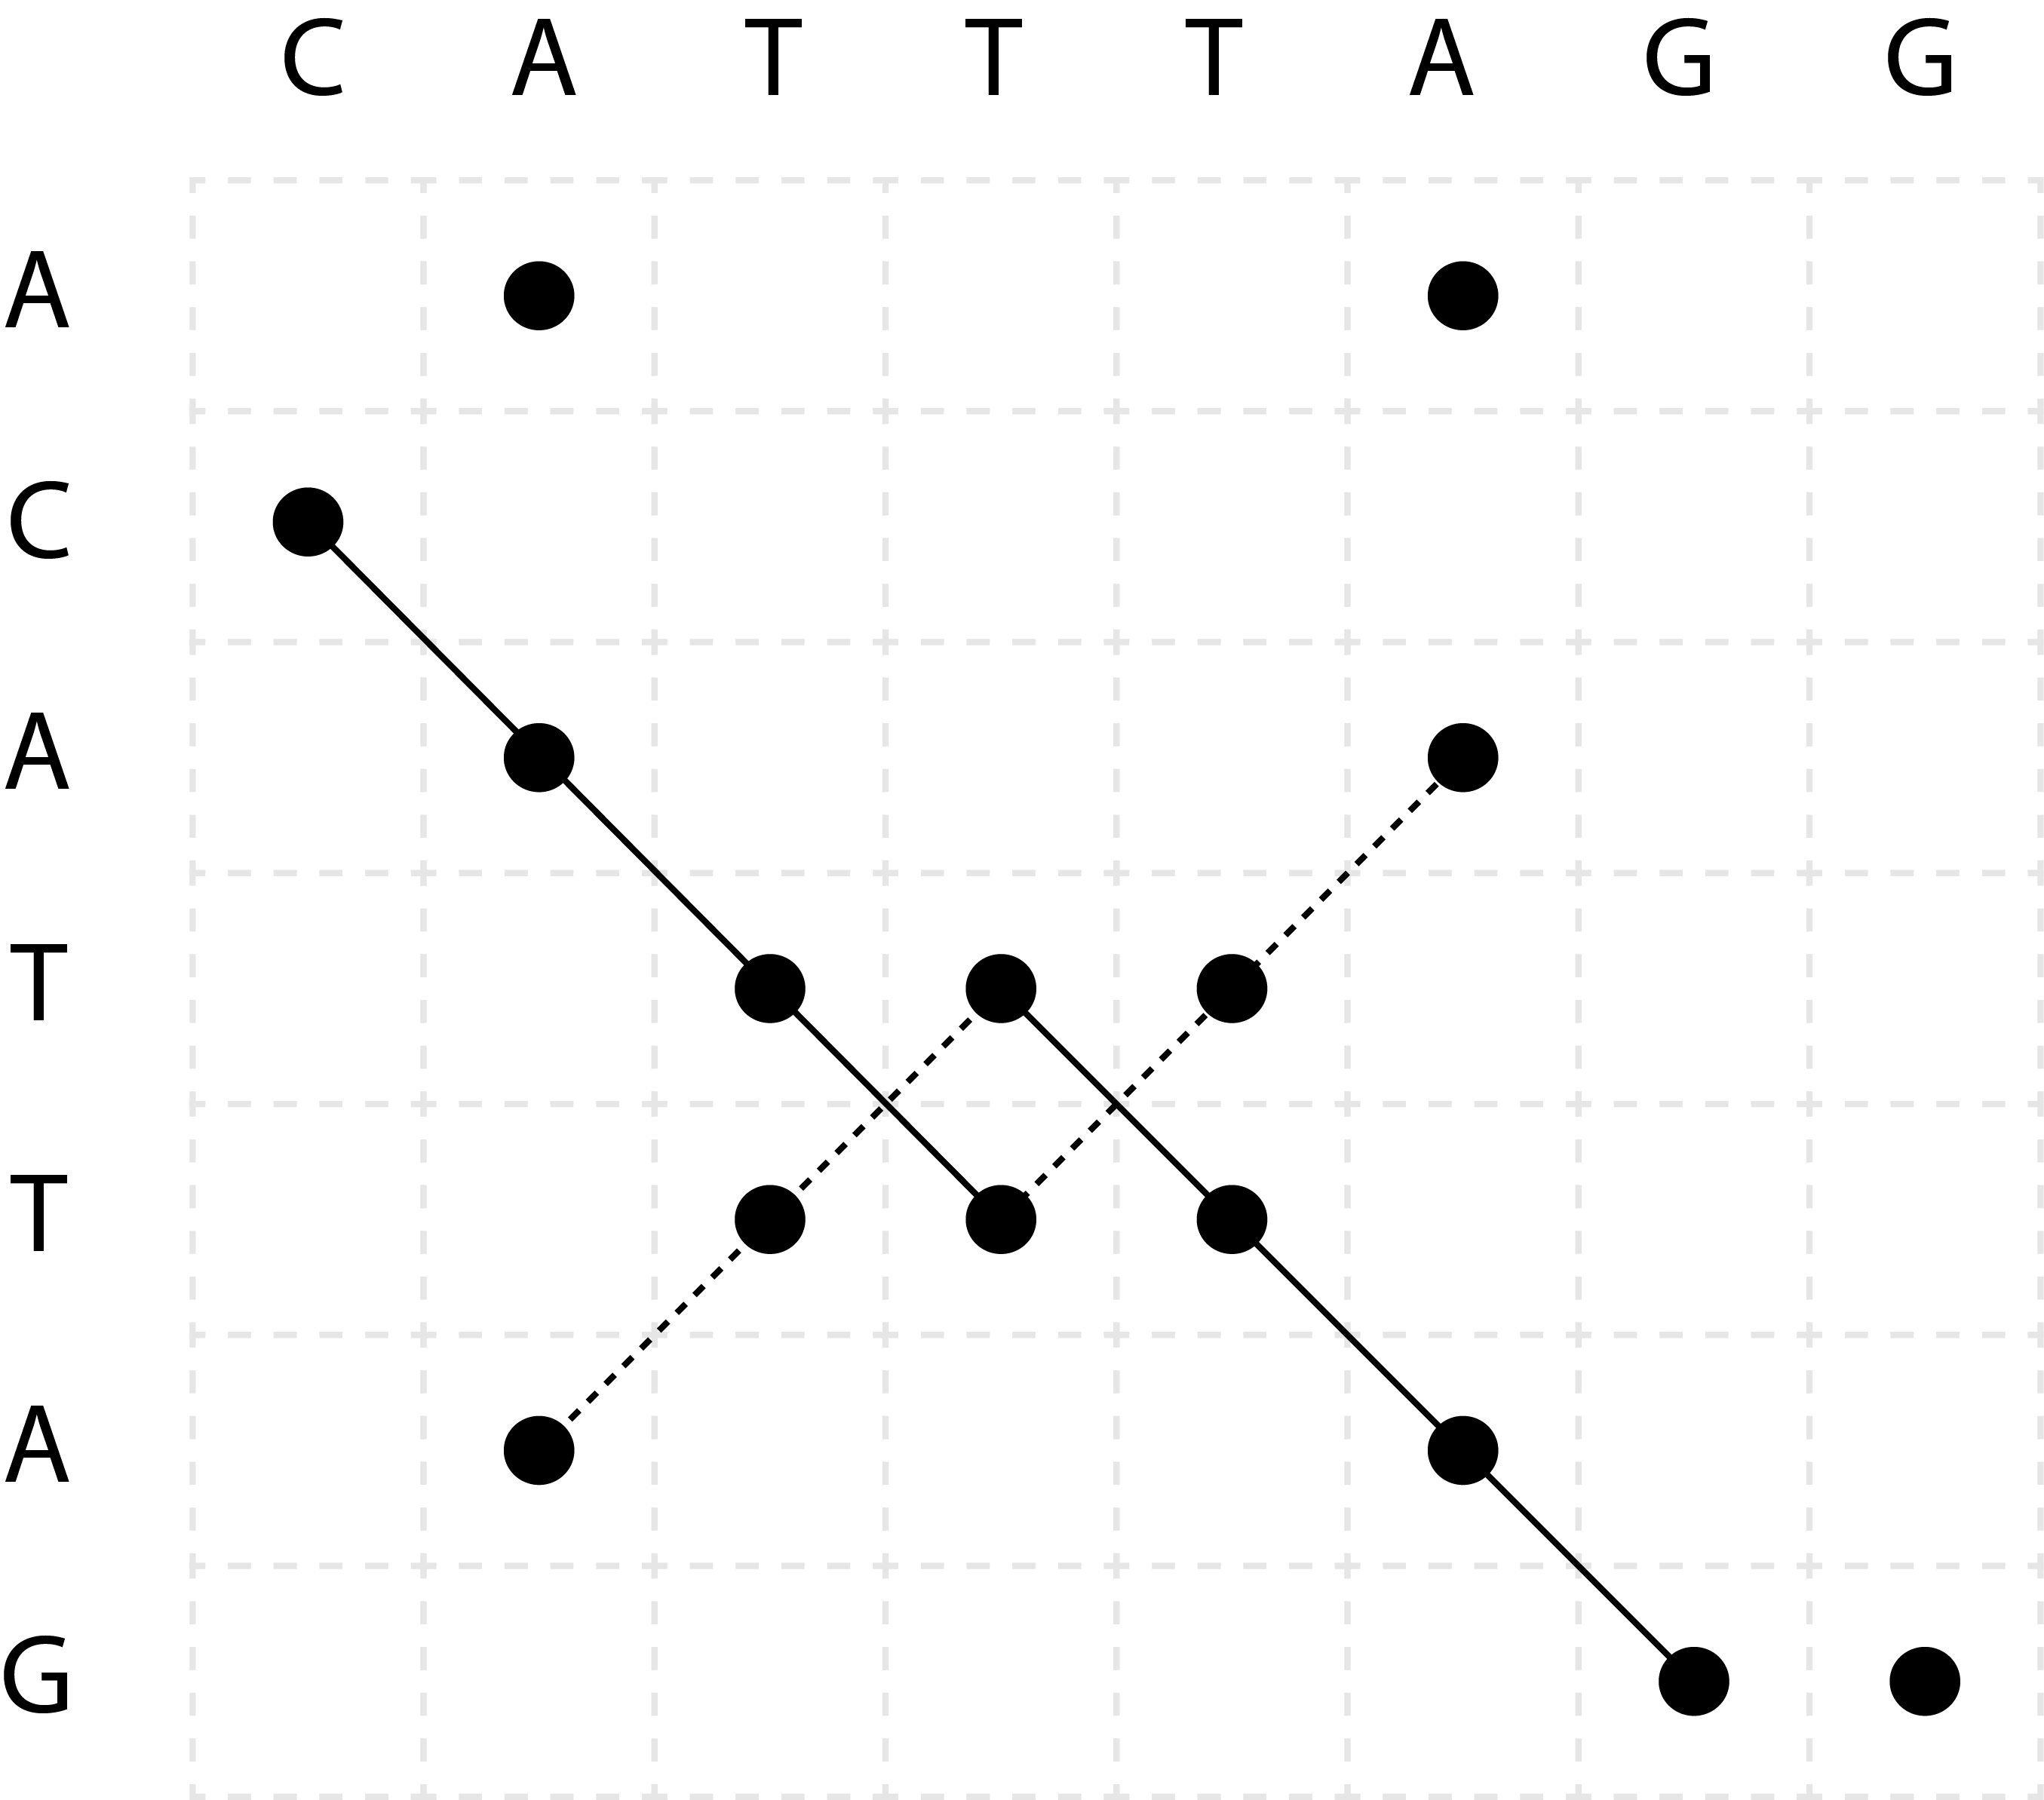
\includegraphics[width=0.3\textwidth]{fig04/dot_matrix.png}
  \caption{Dot matrix of $7 \times 8$}
\end{figure}

\noindent
It is easy to find segment pairs with a dot matrix. Contiguous dots along diagonals indicate local alignments. It is also easy to find other similarities. For instance, contiguous dots along anti-diagonals indicate reversed substrings.

%
% Filtering of dot matrix
%
\subsubsection*{Filtering of dot matrix}
Dot matrices usually get noisy with too many dots.  Overlapping windows are usually applied to reduce the noise.

\bigskip 
\noindent
\textbf{Example of filtering}

\begin{figure}[H]
  \centering
      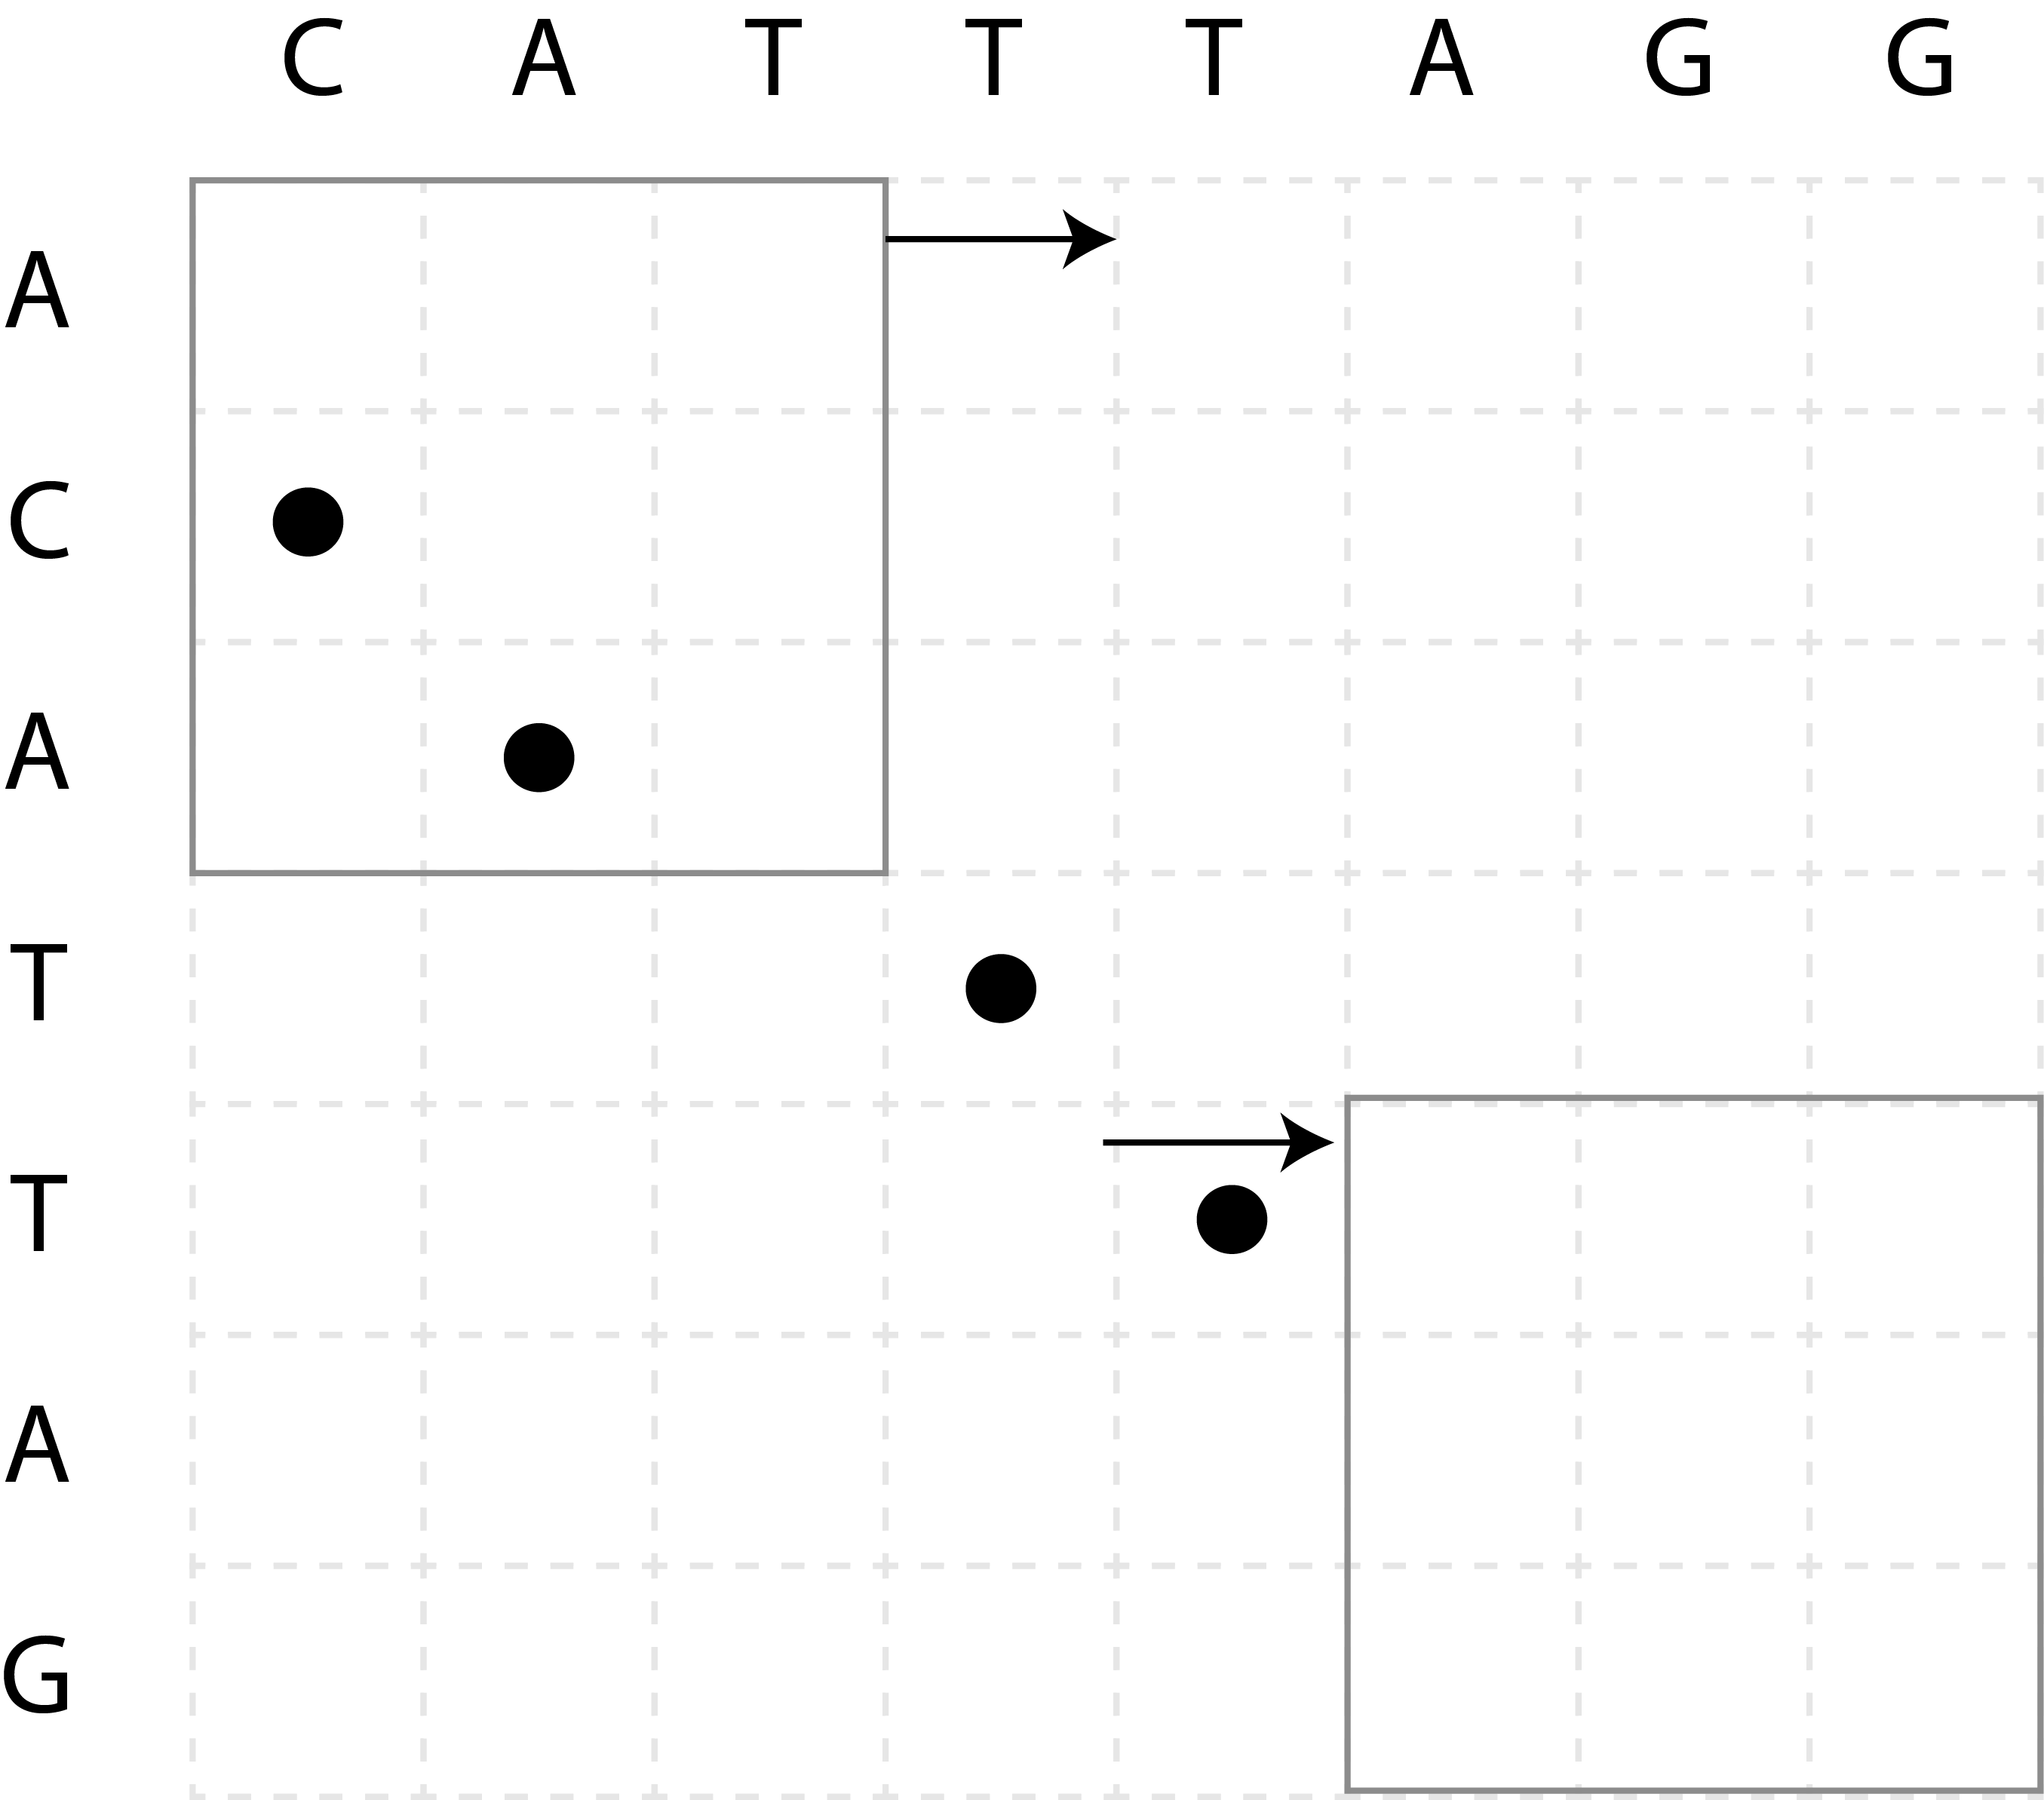
\includegraphics[width=0.3\textwidth]{fig04/dot_matrix_filtered.png}
  \caption{Filtered dot matrix with window size 3 and threshold 3.}
\end{figure}

%
% Exercise \thesection.2
%
\subsubsection*{Exercise \thesection.2}
Find local similarities between two DNA sequences, \verb|q: GATTACA| and \verb|d: GGATTTAC|.

\begin{enumerate}
\item Create a dot matrix for the two sequences.
\item Filter dots with overlapping windows size 3 and threshold 3.
\end{enumerate}

\bigskip 

%\end{document}


\end{document}
